%%%%%%%%%%%%%%%%%%%%%%%%%%%%%%%%%%%%%%%%%%%%%%%%%%%%%%%%%%%%%%%%%%%%%%%%%%%%%
%
%  System        : 
%  Module        : 
%  Object Name   : $RCSfile$
%  Revision      : $Revision$
%  Date          : $Date$
%  Author        : $Author$
%  Created By    : Robert Heller
%  Created       : Mon Sep 25 10:36:02 2017
%  Last Modified : <170925.1435>
%
%  Description 
%
%  Notes
%
%  History
% 
%%%%%%%%%%%%%%%%%%%%%%%%%%%%%%%%%%%%%%%%%%%%%%%%%%%%%%%%%%%%%%%%%%%%%%%%%%%%%
%
%    Copyright (C) 2017  Robert Heller D/B/A Deepwoods Software
%			51 Locke Hill Road
%			Wendell, MA 01379-9728
%
%    This program is free software; you can redistribute it and/or modify
%    it under the terms of the GNU General Public License as published by
%    the Free Software Foundation; either version 2 of the License, or
%    (at your option) any later version.
%
%    This program is distributed in the hope that it will be useful,
%    but WITHOUT ANY WARRANTY; without even the implied warranty of
%    MERCHANTABILITY or FITNESS FOR A PARTICULAR PURPOSE.  See the
%    GNU General Public License for more details.
%
%    You should have received a copy of the GNU General Public License
%    along with this program; if not, write to the Free Software
%    Foundation, Inc., 675 Mass Ave, Cambridge, MA 02139, USA.
%
% 
%
%%%%%%%%%%%%%%%%%%%%%%%%%%%%%%%%%%%%%%%%%%%%%%%%%%%%%%%%%%%%%%%%%%%%%%%%%%%%%

\documentclass[12pt]{article}
\usepackage{times}
\usepackage{url}
\usepackage{graphicx}
\usepackage{mathptm}
\usepackage{makeidx}
\usepackage[pdftex,pagebackref=true]{hyperref}
\hypersetup{%
  colorlinks=true,%
  linkcolor=blue,%
  citecolor=blue,%
  unicode%
}
\title{Broadband MLP Costs With and Without Regionalization}
\author{Robert Heller}
\date{\today}
\makeindex
\begin{document}

\maketitle

\tableofcontents
\listoffigures
\listoftables


\section{Introduction}

This paper will explore what happens to the cost of operating a municipal 
broadband network when one moves from a single town network to a multi-town 
\textit{regional} network.  There seems to be some lack of real understanding 
about what happens to the cost of operating a municipal broadband network in 
the context of a regional network.  It is my contention that for almost all of 
the unserved towns in Western Massachusetts, operating as single town networks 
is not really sustainable, at least not at an \textit{affordable} price.  Only 
one or two towns have any reasonable chance of operating as single town 
network in a sustainable way, but only at prices that are \textit{barely} 
affordable.

I will be using some simple cost assumptions, to perform a simple set of cost
analysis. It is not the intent of this paper to present actual cost
projections or pricing models, since others have done that. I am simply going
to present an analysis of what generally happens to the costs when one moves
from a single town network to a multi-town regional network.  I took the base 
numbers from the Wendell Sustainability Worksheet\cite{WendSustain}.

\section{The Three ``buckets'' of Broadband MLP Costs}

The first thing to understand about the Broadband MLP Costs is that the costs 
fall into three categories (or ``buckets'')\index{Buckets, cost}:

\begin{enumerate}
\item Per subscriber costs.  These are costs that are always the same per 
subscriber no matter how many subscribers there or how many miles of fiber 
there is.  These costs relate mostly to the costs associated with billing and 
customer service.  That is the cost to print and mail the bills, the costs of 
processing the payments.  Also the costs for customer service and technical 
support.
\item Per overall network costs.  These are one-of costs for the overall 
network and are the same for a small network or a large network.  These are 
things like the cost for the accounting, legal, and general insurance fees.
\item Per mile costs.  These are costs that depend on the number of miles of 
fiber\footnote{And also the number of poles.  Since the pole spacing is more 
or less constant, I am using a constant conversion between number of poles and 
number of miles.}.  These include costs like outside plant maintenance costs and 
things like pole rental and pole bond, along with things like the depreciation 
reserve, since that is based on the cost on the fiber.
\end{enumerate}

The first bucket is not affected by the size of the network.  It is also a 
relatively small part of the monthly subscriber fee.  I am going to ignore 
this cost in this paper, since regionalization has no effect on this part of 
the monthly subscriber fee.

The second bucket is most interesting, since it is generally unaffected by the 
size of the network, large or small.  The portion of the subscriber fee that 
covers these costs goes down as the number of subscriber increases.

The third bucket is less interesting, but worth looking at.  The portion of 
the subscriber fee that covers these costs goes down as the \textit{density} 
of subscribers increases.

\section{Typical ``single town'' Broadband MLP Costs}

\begin{figure}[Hptb]
\begin{centering}
\includegraphics[width=5in]{WENDELL-PerMile.pdf}
\caption{Wendell Per Mile costs}
\label{fig:WENDELLPM}
\end{centering}
\end{figure}
\begin{figure}[Hpbt]
\begin{centering}
\includegraphics[width=5in]{WENDELL-PerNetwork.pdf}
\caption{Wendell Per Network costs}
\label{fig:WENDELLPN}
\end{centering}
\end{figure}

\clearpage

Figures~\ref{fig:WENDELLPM} and \ref{fig:WENDELLPN} show how the costs work
out for the Town Of Wendell as a single town network. The vertical red lines
show Wendell's total subscriber base and the average subscriber density. The
black line on the graphs show the subscriber fee for a range of total
subscriber count and subscribers per mile. The area above and to the right of
the black line is ``operating in the black'' and represents excess revenue
(``profits'') and the area below and to the left of the black line is
``operating in the red'' and and represents losses. Operating exactly on the
black is just breaking even. The blue line is a ``goal'' subscriber fee, what
one might consider what the subscriber can afford for this cost. The red lines
represent that actual total number of subscribers and the actual subscriber
density. The intersection of the red and blue lines tell us where we are in
terms of sustainability. We want that int erection to land somewhere so that we
are at least breaking even, if not with a profit. The thing to note here is
that at an \textit{affordable} subscriber fee, Wendell just does not have
enough subscribers to be sustainable\footnote{Effectively, Wendell ``lied''
(with the help of MBI!) on our readiness assessment by simply assuming that a
higher subscriber fee was actually going to be affordable. I expect that most
towns did this.}.

\begin{figure}[Hptb]
\begin{centering}
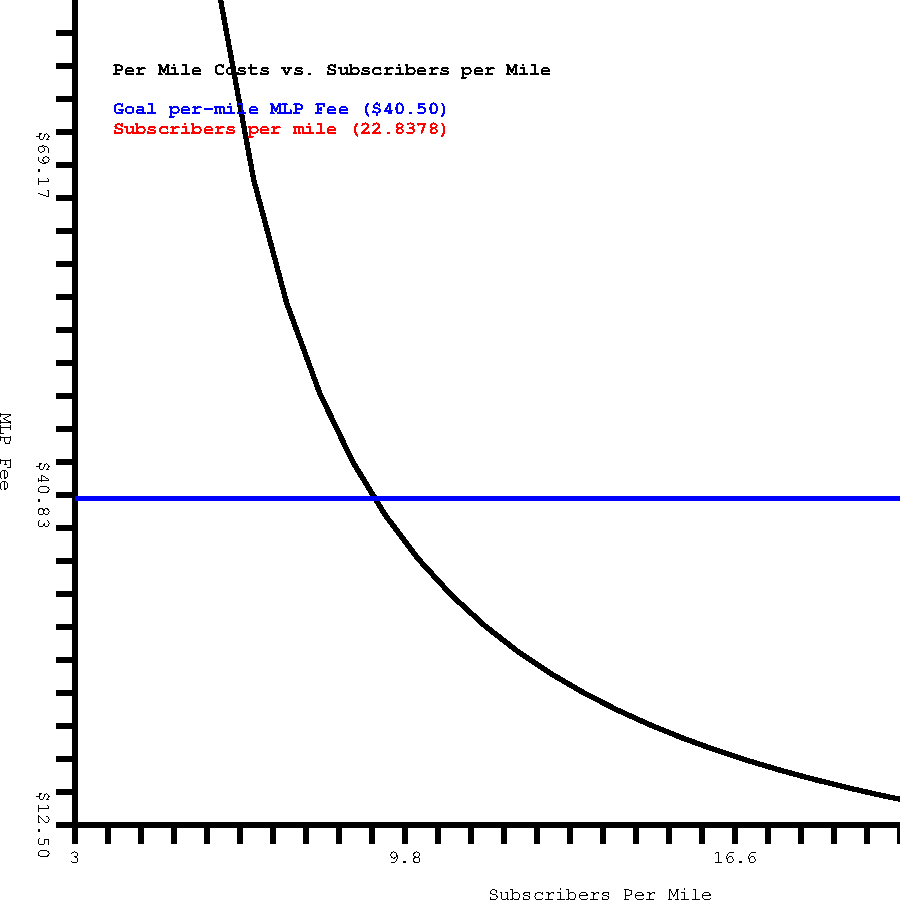
\includegraphics[width=5in]{SHUTESBURY-PerMile.pdf}
\caption{Shutesbury Per Mile costs}
\label{fig:SHUTESBURYPM}
\end{centering}
\end{figure}
\begin{figure}[Hpbt]
\begin{centering}
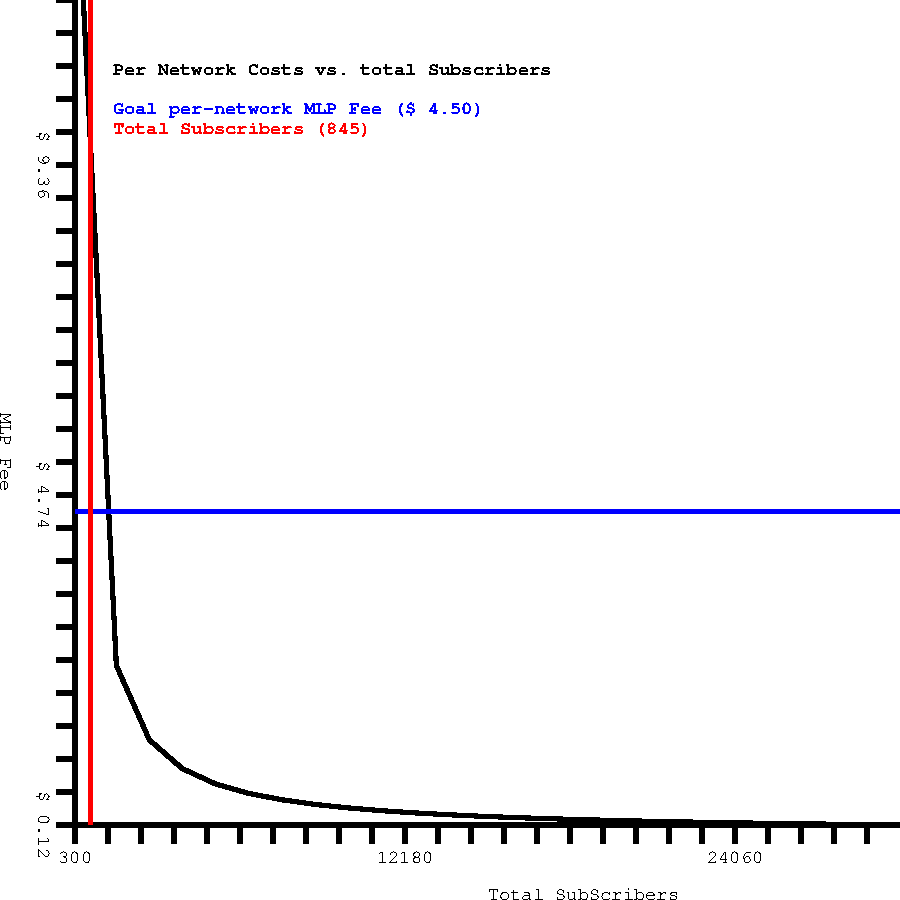
\includegraphics[width=5in]{SHUTESBURY-PerNetwork.pdf}
\caption{Shutesbury Per Network costs}
\label{fig:SHUTESBURYPN}
\end{centering}
\end{figure}

\clearpage

Figures~\ref{fig:SHUTESBURYPM} and \ref{fig:SHUTESBURYPN} show how the costs
work out for the Town Of Shutesbury as a single town network. The vertical red
lines show Shutesbury's total subscriber base and the average subscriber
density.  Shutesbury, being more populous does a lot better, but even 
Shutesbury is on the edge of not being sustainable.  The much higher density 
helps a lot, but it is a little iffy.  


\section{What happens to the Broadband MLP Costs when the network is 
regionalized}

\begin{figure}[Hptb]
\begin{centering}
\includegraphics[width=5in]{NEW_SALEM-SHUTESBURY-WENDELL-PerMile.pdf}
\caption{New Salem, Shutesbury, and Wendell Per Mile costs}
\label{fig:NEWSALEM-SHUTESBURY-WENDELLPM}
\end{centering}
\end{figure}
\begin{figure}[Hpbt]
\begin{centering}
\includegraphics[width=5in]{NEW_SALEM-SHUTESBURY-WENDELL-PerNetwork.pdf}
\caption{New Salem, Shutesbury, and Wendell Per Network costs}
\label{fig:NEWSALEM-SHUTESBURY-WENDELLPN}
\end{centering}
\end{figure}
\begin{figure}[Hptb]
\begin{centering}
\includegraphics[width=5in]{BECKET-GOSHEN-HEATH-NEW_ASHFORD-NEW_SALEM-PLAINFIELD-ROWE-SHUTESBURY-WASHINGTON-WENDELL-WINDSOR-PerMile.pdf}
\caption{11 town Per Mile costs}
\label{fig:BECKET-GOSHEN-HEATHETCPM}
\end{centering}
\end{figure}
\begin{figure}[Hpbt]
\begin{centering}
\includegraphics[width=5in]{BECKET-GOSHEN-HEATH-NEW_ASHFORD-NEW_SALEM-PLAINFIELD-ROWE-SHUTESBURY-WASHINGTON-WENDELL-WINDSOR-PerNetwork.pdf}
\caption{11 town Per Network costs}
\label{fig:BECKET-GOSHEN-HEATHETCPN}
\end{centering}
\end{figure}

\clearpage

But look what happens with a very modest 3 town regional network (New Salem,
Shutesbury, and Wendell). Figures~\ref{fig:NEWSALEM-SHUTESBURY-WENDELLPM} and
\ref{fig:NEWSALEM-SHUTESBURY-WENDELLPN} show that merely increasing the total
subscriber base moves the red line just into the profitable region, if only
slightly. Going to an 11\footnote{Becket, Goshen, Heath, New Ashford, New
Salem, Plainfield, Rowe, Shutesbury, Washington, Wendell, and Windsor.} town
network gives us a massive improvement, as shown in
Figures~\ref{fig:BECKET-GOSHEN-HEATHETCPM} and
\ref{fig:BECKET-GOSHEN-HEATHETCPN}.

\section{Conclusions}

The conclusion I have drawn from this exercise is that to achieve sustainability
at an affordable price one needs to maximize the customer base and to work
with as dense a customer base as possible, although density of the customer
base is actually less of an issue. When the size of the customer base grows to
the point of passing the ``knee'' of the graph, sustainability \textit{and}
affordability can be easily ac hived and with a comfortable margin (allowing
spare revenue for various sorts of ``disasters''). Most of the small towns in
our region are actually so small that getting past the knee is essentially
impossible and the only want to cover the cost of most single town networks is
to set the subscriber price so high as to make it unaffordable to most of the
people in our region.

\appendix

\section{Methodology}

To generate the graphs used in this paper, I wrote a Tcl/Tk 
program\cite{MLPCostGraphs}.  I have uploaded the source code to a GitHub 
repository(\url{http://www.github.com/RobertHeller/}).  I have also uploaded 
ready-to-run binaries of the program for various operating system to my 
company website at this web address: \url{http://www.deepsoft.com/}.  People 
who are interested can download the program and use it to try it out with 
various parameter settings and various regional network scenarios.

\clearpage
\addcontentsline{toc}{section}{References}
\bibliography{MLPCostsWithRegionalization}
\bibliographystyle{plain}
\clearpage
\addcontentsline{toc}{section}{Index}
\printindex


\end{document}

